
\section{Grundlagen}
\label{sec:Grundlagen}
\subsection{Einleitung}

\subsection{Genetische Algorithmen}

\subsection{Aufbau eines GA in Einzelschritten}
\subsubsection{Initzialisierung der Population}
\subsubsection{Grade}
\subsubsection{Evolve}
\paragraph{Select Parents}
\paragraph{Breed}
\paragraph{Exchange}
\subsection{Loop}


\subsection{K"unstliche Neuronale Netze}
\begin{figure}[htb]
  \centering  
  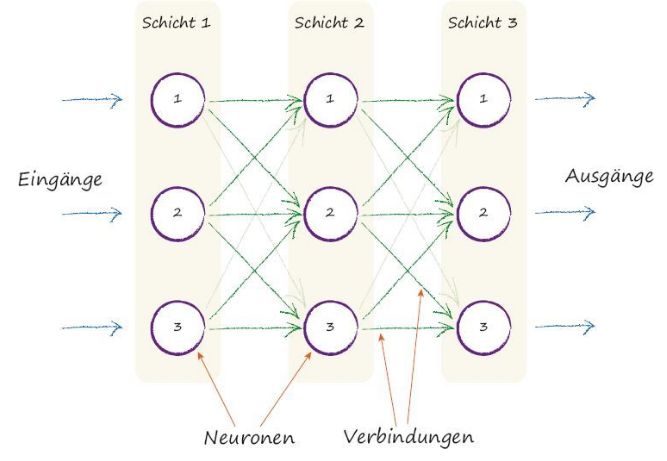
\includegraphics[scale=0.5]{img/S36_Buildyourown.png}
  \caption{Neuronales Netz   \cite{rashid2017neuronale}}
  \label{fig:neural_network}
\end{figure}

Zu sehen ist ein Künstliches Neuronales Netz mit drei Schichten \ref{fig:neural_network}. Dies wurde dem natürlichen Vorbild der neuronalen Netze im Gehirn nach empfunden. Die Kreise nennt man Neuronen, mehrere Neuronen zusammen ergeben eine Schicht oder auch Layer genannt. Die Verbindungen sind die Gewichte, so kann einem Netz verschiedene Zusammenhänge von Input und Output antrainiert bzw. angelernt werden. Zum Training werden viele Daten benötigt, aus welchen das Netz \glqq Lernt\grqq{}. Dafür ist es wichtig, viele aufbereitete Daten zu besitzen, denn diese Netze brauchen viele Trainingsiterationen, bis das gewünschte Ergebnis zustande kommt. Ein Neuron besteht aus Eingängen, Gewichten und einer Aktivierungfunktion sowie einem Ausgang. Die Vernetzung mehrerer Neuronen lässt ein Neuronales Netz entstehen.

\newpage
\subsection{Aufbau eines Neurons}
\begin{figure}[htb]
  \centering  
  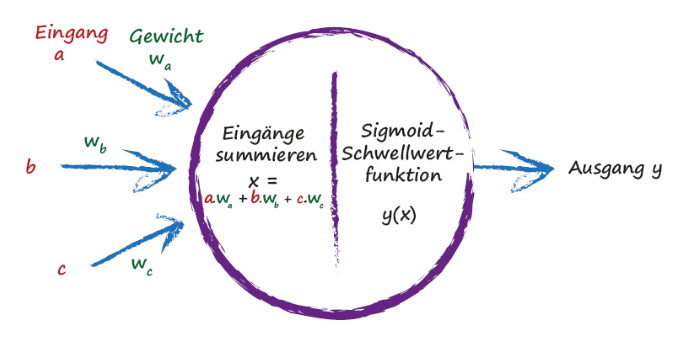
\includegraphics[scale=0.5]{img/S41_Buildyourown.png}
  \caption{Aufbau eines Neurons  \cite{rashid2017neuronale}}
  \label{fig:neuron}

\end{figure}
\subsubsection{Input}
Der Input wird mit den einzelnen Gewichten verrechnet, anschließend werden diese zusammen gebracht. Diese Werte werden zufällig initialisiert und per Training verbessert, somit handelt es sich um einen angelernten Werte, welche durch die Backproagation (Fehlerrückführung) verbessert werden.

\subsubsection{Bias}
Auf diesen Input wird anschließend ein Bias gerechnet, dieser führt zu einem besseren Verhalten beim Trainieren. Bei diesen Werten handelt es sich um angelernte Werte, die per Backpropagation verbessert werden und die Flexibitlität der Netze erhöht.


\subsubsection{Activation Function}
Die Aktivierungsfunktion kann man sich als Schwellwert vorstellen, ab wann das Neuron den Input weiter gibt. Es gibt verschiedene Funktionen, um diesen Schwellwert zu definieren. Bei Klassifizierungen werden heute meist ReLu-Layer oder ein Weakly-ReLu Layer benutzt, diese verhindern das Vanishing- bzw. Exploding- gradientproblem beim Trainieren.

\subsubsection{Output}
Wenn der Schwellwert überschritten wird, wird am Output durchgeschaltet.
Von Input nach Output nennt sich ein Single-Forward-Pass. Wie hier beschrieben wird, kann ein Netz verschieden viele Layer besitzen mit verschiedenen Anzahlen von Neuronen.

\subsection{Lossfunction}
Die Verlustfunktion stellt ein ausgesuchtes Maß der Diskrepanz zwischen den beobachteten und den vorhergesagten Daten dar. Sie bestimmt die Leistungsfähigkeit des neuronalen Netzes während des Trainings und der Ausführung. Ziel ist es, im laufenden Prozess der Modellanpassung, die Verlustfunktion zu minimieren.

\subsection{Backpropagation}
Um die Fehlerfunktion zu minimieren wird als Tool Gradienten Abstieg benutzt. Im Grunde werden dabei die Gewichte so angepasst, dass ein besseres Ergebnis entsteht und dadurch die Fehlerfunktion verringert wird. Wie das Wort Backpropagation schon sagt, wird von hinten nach vorne verbessert. Es gibt verschiedene Variationen von Gradientenabstiegen, welche verschiedene Vor- und Nachteile haben. Bei dem Trainieren des Netzes wurde der Momentum-Optimizer, welcher aus einem Gradientenabstieg mit Momentum aufgebaut ist.

\subsection{Hyperparameter}


\subsection{Learning Methods}

\subsubsection{Supervised Learning}
Überwachtes Lernen wird dafür benutzt, eine Funktion zu finden, Daten einem Wert zuzuweisen. Dennoch müssen dafür alle Daten vorverarbeitet werden und einem Label zugeordnet werden. Damit das Netz auch eine Aussage über das Ergebnis, während des Trainings, geben kann. Anwendungsfälle sind Regression, Klassifikation und Empfehlungen.

\subsubsection{Unsupervised Learning}
Im Vergleich zum überwachten Lernen liegen hier keine Labelinformationen vor. Weshalb dieser Ansatz eher zum Erkennen von Mustern und Ableiten von Regeln da ist. Für unsupervised Leaning Algorithem sind in der Regel sehr viele Daten nötig. Anwendungsgebiete sind das Clustering und die Dimensionsreduktion.
